\documentclass[aps,prb,twocolumn,
	           groupedaddress,superscriptaddress,
               amsfonts,amssymb,amsmath,floatfix,
	           citeautoscript]{revtex4-1}


% --- PACKAGES ---
\usepackage{graphicx}
\usepackage[centering,hmargin=20mm,tmargin=30mm,bmargin=25mm]{geometry}
\usepackage{multirow}
\usepackage{newtxtext}
\usepackage[cmintegrals]{newtxmath}

%-----SI UNITS-----
\usepackage{siunitx}
\sisetup{range-phrase =\text{\,--\,},
	list-units   =single,
	range-units  =single,
	list-pair-separator = {\ \text{and}\ },
	list-separator = {,\ \linebreak[0]},
	list-final-separator = {,\ \linebreak[0]\text{and}\ }}

%--- REFERENCING ---
\usepackage{xcolor}
\usepackage{hyperref}
\hypersetup{colorlinks,
	linkcolor={blue!75!black!80!yellow},
	citecolor={blue!75!black!80!yellow},
	urlcolor={blue!75!black!80!yellow}
}

%--- CAPTIONS (sans serif) ---
\makeatletter
\renewcommand\@make@capt@title[2]{%
	\@ifx@empty\float@link{\@firstofone}{\expandafter\href\expandafter{\float@link}}%
	\sffamily{\textbf{#1}}\@caption@fignum@sep#2
}%
\renewcommand\figurename{Figure}
\makeatother

% --- SPACING ---
\usepackage{microtype} % Kerning and symbol-stretching
\usepackage{xspace}

\thickmuskip=5mu plus 2mu minus 1mu  %binary relations (default, 5mu plus 5mu)
\medmuskip=4mu plus 2mu minus 2mu    %binary operations (default, 4mu plus 2mu minus 4mu)

\frenchspacing %Ensure that revTeX does not do "double spaces" after punctuation

% --- COMMANDS ---
\renewcommand{\Im}{\operatorname{Im}}
\renewcommand{\Re}{\operatorname{Re}}
\newcommand{\sgn}{\operatorname{sgn}}

\newcommand{\iu}{\mathrm{i}}
\newcommand{\e}{\mathrm{e}}
\newcommand{\dd}{\mathrm{d}}
\newcommand{\unitvec}[1]{\ensuremath{\hat{\mathbf{#1}}}}
\newcommand{\sub}[1]{\ensuremath{_{\textrm{#1}}}} %Upright multi-character subscript
\newcommand{\super}[1]{\ensuremath{^{\textrm{#1}}}} %Upright multi-character superscript

%abbreviations
\newcommand{\ie}{i.e.\@\xspace} %Gobble-spaces of the "small" type (small is ensured by adding \@)
\newcommand{\cf}{cf.\@\xspace}
\newcommand{\eg}{e.g.\@\xspace}
\newcommand{\etc}{etc.\@\xspace}

\newcommand{\HarvardSEAS}{John A. Paulson School of Engineering and Applied Sciences, Harvard University, Cambridge, MA, USA}
\newcommand{\MITPhy}{Department of Physics, Massachusetts Institute of Technology, Cambridge, MA, USA}

% ----- COMMENTS AND META-ANNOTATIONS -----
\usepackage{textcomp} % for \textrightarrow
\usepackage{xifthen}
\usepackage{etoolbox}
\newboolean{togglecomments}
\newboolean{togglechanges} 

% toggle to true to see comments (otherwise hidden)
\setboolean{togglecomments}{true}  
% toggle to false to see mixed versions (otherwise edits are shown exclusively)
\setboolean{togglechanges}{false} 

\newcommand{\comment}[2]{%
    \ifbool{togglecomments}%
    {\textcolor{blue!70!black}{\small\textsf{%
    \textsuperscript{\textsc{\textsf{\MakeLowercase{#1}}}}%
    [#2]}}} % if true, show comments
    {}}     % if false, do nothing
\newcommand{\swap}[2]{\ifbool{togglechanges}
    {#2}  % TC-only version
    {\textcolor{red!70!black}{[#1]}\text{\textrightarrow{}}\textcolor{green!50!black}{[#2]}}}
\newcommand{\remove}[1]{\ifbool{togglechanges}
    {}    % TC-only version
    {\textcolor{red!70!black}{#1}}}
\newcommand{\inset}[1]{\ifbool{togglechanges}
    {{}#1}  % TC-only version
    {\textcolor{green!50!black}{{}#1}}}
\makeatletter
\newcommand{\citeremind}[1]{%
	\unskip%
    \textcolor{blue!75!black!80!yellow}{${}^\blacksquare$%
	\ifthenelse{\isempty{#1}}{}{\textsuperscript{\tiny\textsf{#1}}}%
	}\xspace}
\makeatother
\newcommand{\FIXME}[1]{\textcolor{red!70!black}{[#1]}}
\newcommand{\optional}[1]{\textcolor{yellow!70!gray}{#1}}





% --- DOCUMENT ---
\begin{document}

% --- TITLE & AUTHORSHIP ---
\title{Nanophotonics with optical phonons in two dimensions}

\author{Nicholas Rivera}
\email{nrivera@seas.harvard.edu}
\affiliation{\HarvardSEAS}\affiliation{\MITPhy}
%
\author{Thomas Christensen}
\affiliation{\MITPhy}
%
\author{Prineha Narang}
\email{prineha@seas.harvard.edu}
\affiliation{\HarvardSEAS}

\date{\today}

% --- ABSTRACT ---
\begin{abstract}
    Extreme confinement of electromagnetic energy by phonon-polaritons \swap{promises}{holds the promise of} extremely strong and novel forms of control over the dynamics of matter. 
    To bring such control to its ultimate limit, it is important to consider phonon-polaritons in two dimensional systems. 
    \comment{tc}{It is not necessarily clear to me why 2D phonon-polaritonics would be an obvious component in bringing phonon-polaritons to their ``ultimate limit''?}
    Recent studies have pointed out that in two-dimensional systems, splitting between longitudinal and transverse optical (LO and TO) phonons is absent at the $\Gamma$ point.  
    Does this lack of LO--TO splitting imply the \swap{lack}{absence} of a \swap{strongly confined electromagnetic (phonon-polariton) mode}{phonon-polariton} in polar monolayers? 
    Here, we derive a universal form for the spatially-nonlocal dielectric function of a polar monolayer specified by: the TO phonon frequency, the non-zero group velocity of the LO phonon, and the phonon lifetime. 
    \comment{tc}{I'm a bit hesitant to highlight the ``spatially-nonlocal'' dielectric function: the real reason this (simplified) form is nonlocal is just dimensional---\eg graphene's dielectric function is also nonlocal in a similar fashion (even in the low-momentum, low-frequency limit). The associated surface conductivity is local; so the in-plane polarization response is also local.} 
    Our analysis reveals that the phonon-polariton of the bulk is \swap{``replaced''}{essentially supplanted/replaced} by the LO phonon\inset{ of the two-dimensional system}.
    We \swap{present}{discuss} the confinement and propagation losses of the LO \swap{phonons}{phonon-polaritons}, finding that high \remove{LO phonon} confinement and reasonable propagation quality factors coincide in regions which are difficult to detect with current near-field optical microscope techniques. 
    We conclude by studying the interaction of external emitters with two-dimensional hBN nanostructures, finding extreme enhancement of spontaneous emission due to \swap{2D phonon channels}{coupling with localized 2D phonon-polaritons}, and the possibility of multi-mode strong and ultra-strong coupling between an external emitter and hBN \swap{phonons}{phonon-polaritons}.
\end{abstract}

\maketitle

\comment{tc}{Both `phonon-polaritons' and `phonon polaritons' are used; let's settle on one.}

\comment{tc}{For title, how about `Phonon polaritons in two-dimensional hexagonal boron nitride'?}


% --- INTRODUCTION ---
Phonon polaritons, hybrid quasiparticles of photons and optical phonons supported in polar materials, \swap{offer}{hold} great promise for deeply sub-diffractional control of electromagnetic fields at mid-\swap{IR}{infrared} and \swap{THz}{terahertz} frequencies. \swap{P}{Qualitatively, p}honon polaritons share many features in common with plasmon polaritons in conductors. \swap{In}{E.g., in} recent years, it has been shown that phonon-polaritons enable confinement of light to volumes over $10^6$ times smaller than that of a diffraction-limited photon in free-space\cite{caldwell2013low,xu2014mid,caldwell2014sub,dai2014tunable,tomadin2015accessing,yoxall2015direct,li2015hyperbolic,dai2015subdiffractional,dai2015graphene,caldwell2015low,li2016reversible,Basov:2016,basov2017towards,low2017polaritons,giles2017ultra,li2018infrared,ma2018plane}. Due to this remarkable confinement and their relatively high lifetimes of around picoseconds, phonon-polaritons open new opportunities for vibrational spectroscopy,\citeremind{} radiative heat transfer~\cite{hillenbrand2002phonon}, and control of dynamics in quantum emitters~\cite{kumar2015tunable,rivera2017making,kurman2018control}. 
In many cases, extreme confinement of phonon polaritons is achieved by the use of thin-films, which \swap{shrink}{reduce} the in-\remove{plane} and out-of-plane wavelength of polaritons monotonically with decreasing film thickness~\cite{dai2014tunable,dubrovkin2018ultra}. 
\comment{tc}{The previous and following sentences both start with `many cases' here; best to rewrite one (probably the latter).}
In many cases, a monolayer is the ultimate limit of this effect. Thus, to bring these classical and quantum nanophotonics applications to their ultimate limits, it is necessary to consider the properties of these modes in two-dimensions. 
\comment{tc}{I'm not sure that starting with `however' in this sentence is optimal: we want to convey an additional motivation for studying them (specifically, the transition from 3D to 2D is nontrivial)---maybe this sentence could be rewritten with this perspective in mind.}
However, this picture of monolayers supporting maximally confined phonon-polariton modes is ostensibly complicated by the fact that in two-dimensional polar materials, the LO--TO splitting that gives rise to phonon-polaritons in three-dimensions is absent at the $\Gamma$ point~\cite{sanchez2002vibrational,mele2002electric,serrano2007vibrational,sohier2017breakdown}.

In this Letter, we develop \swap{core results in}{a framework and a several concrete examples for understanding the} the nascent field of optical phononics in two-dimensional materials\swap{ by deriving}{. We do so by deriving} a universal form for the dielectric function of a polar monolayer, \swap{incorporating spatially nonlocal effects}{including spatial nonlocality}, which \swap{is specified fully in terms of the dispersion relation of LO and TO phonons in two dimensions}{which depends solely on the LO and TO phonon frequencies---and their dispersion with momentum---in the two-dimensional system}.
Using parameters from Ref.~\citenum{sohier2017breakdown} for \swap{ important monolayers such as }{the canonical two-dimensional polar monolayer---}hexagonal boron nitride\swap{, }{---}we present the confinement and propagation losses of \swap{these modes}{the supported phonon-polaritons}, identifying the frequency region where they should be most easily detected. \swap{We then}{Finally, we} show that these modes \swap{essentially provide the ultimate limit of}{enable extreme} light-matter interaction between emitters and polar materials, showing that for atom-like emitters, their spontaneous decay can be enhanced by up to eight orders of magnitude by the emitter--LO phonon coupling\swap{, which due to}{. Given} the narrow bandwidth of phonon-polariton resonances, \swap{can lead to }{this suggests} the possibility of realizing the multi-mode strong coupling and ultra-strong coupling regimes of quantum electrodynamics \swap{for an external emitter coupled with optical phonons in hexagonal boron nitride}{in a two-dimensional hexagonal boron nitride platform}. 


% -----------------
\section{Electrodynamics of optical phonons in two-dimensions}
\comment{tc}{Structurally, this section would benefit from being split into two sections: one solely tasked with deriving/establishing the forms of the (non-interacting) polarization-polarization response function---and possibly its equivalent conductivity; and another one solely tasked with deriving and discussing the dispersion relation for the associated longitudinal optical modes. Right now, this section goes back and forth between the two, which (I think) reduces its focus and gives way for unnecessary repetition.}

In this section, we develop \swap{the}{a} theory of electromagnetic \swap{waves associated with}{response due to} optical phonons in two\swap{ dimensions}{-dimensional systems}. The crux of the theory \swap{is determining}{involves} the dielectric \swap{permittivity}{function} associated with the monolayer. 
\swap{It is obtained by considering the response of the ions in the monolayer to a longitudinal electromagnetic wave whose electric field is the gradient of a scalar potential $\phi$.}{To obtain it, we consider the response of the ions of the monolayer due(/when subjected) to a longitudinal electromagnetic potential $\phi$}. The \swap{coupling}{interaction} Hamiltonian is \swap{then given by}{in this case simply}
\begin{equation}
    H_{\mathrm{int}} = \int \dd^2x ~\rho \phi = -\int \dd^2x~ (\nabla\cdot\mathbf{P})\phi,
    \label{eq:coupling}
\end{equation} 
with $\rho$ the \inset{induced} charge density and $\mathbf{P}$ the \inset{total} polarization density associated with the ionic motion. 
\swap{The polarization \inset{density} can be expanded in powers of the displacement of the ions. In particular, we can consider the polarization $P_i$ generated in the monolayer when atom $\kappa$ of the unit cell is displaced along the $j$ direction by amount $u_{\kappa,j}$. To lowest order:}{Within linear response, the induced polarization density can be straightforwardly evaluated from the displacement amplitude $\mathbf{u}_{\kappa}$ of every atom $\kappa$ within the unit cell. Specifically, to first-order, the induced polarization is:}
\comment{tc}{I don't see how the second equality can be consistent: since, by Taylor expansion, $P_i = P_i^0 + u_{\kappa,j}\partial_{u_{\kappa,j}}P_i + \mathcal{O}(u_{\kappa,j}^2)$---so where does the unit cell area $\Omega$ come from? The issue seems to arise from alternatingly interpreting the LHS/RHS $P_i$ as total/density quantities. The right-most equation also seems to be missing a $\kappa$-subscript in $u_{j}$.}
\begin{equation}
    P_i - P_i^{0} = \Omega\frac{\partial P_i}{\partial u_{\kappa,j}}u_{\kappa,j} \equiv Z_{\kappa,ij}u_{j},
\end{equation} 
where $Z_{\kappa,ij}$ is the Born effective charge tensor of ion $\kappa$ and $\Omega$ is the unit cell area.
\comment{tc}{We do not give a definition of $P_i^0$: we also do not comment on what the implications are if it is nonzero (it could be..!)---as far as I can see, we are assuming it is zero for the remaining analysis.}
With this relation between polarization and ionic displacements, \swap{we have expressed the Hamiltonian as a coupling between the scalar potential and ionic displacements}{the interaction Hamiltonian in Equation~\eqref{eq:coupling} couples the scalar potential and the ionic displacements}. 
We consider the response of the monolayer to a scalar potential of the form $\phi\inset{(\mathbf{r})} = \phi(\mathbf{q},\omega)\e^{\iu\mathbf{q}\cdot\mathbf{r}-\iu\omega t}$, where $\mathbf{q}$ is a two-dimensional wavevector in the plane of the monolayer. Such a potential corresponds to a longitudinal electric field \remove{of the form} $\mathbf{E}\inset{(\mathbf{r})} = \iu\mathbf{q}\swap{\phi(\mathbf{q},\omega)\e^{\iu\mathbf{q}\cdot\mathbf{r}-\iu\omega t}}{\phi(\mathbf{r})}$. 
\comment{tc}{I don't think it really ``follows'' from the preceding that $P_i = ... E_{j,\text{tot}}(\mathbf{q},\omega)$. First, this specializes to the RPA via a mean-field approximation, and second, it introduces a response function (so, really, it is more of a definition). It is probably better to phrase these next few sentences rather carefully and with specificity, \eg with references to the usual Kubo formula/approach etc. It may also make sense to split the $P_i = ... E_{j,\text{tot}}(\mathbf{q},\omega)$ off onto its own line, since this is the equation that lends practical utility to the $\boldsymbol{\Pi}$ response function. 
Finally, I don't think we actually need to mention the RPA or anything like it at this point: so far, this is just the non-interacting polarization-polarization response---we effectively arrive at the RPA later on, when we start doing electromagnetic calculations (\ie around Eq.~\eqref{eq:2dmaxwell}); only then do we actually make use of $\mathbf{P} \propto \boldsymbol{\Pi}\mathbf{E}_{\mathrm{tot}}$.}
It follows that the induced polarization takes the form $P_i\inset{(\mathbf{q})}  = \epsilon_0\Pi_{ij}(\mathbf{q},\omega)E_{j,\mathrm{tot}}(\mathbf{q},\omega)$, where $\Pi_{ij}(\mathbf{q},\omega)$ is the polarization-polarization response function of the monolayer and  $E_{j,\mathrm{tot}}(\mathbf{q},\omega)$ is taken as the \textit{total} field which is a sum of the applied field and the field created by induced polarization. The polarization-polarization response function is given by
\begin{equation}\label{eq:2dsusceptibility}
    \boldsymbol{\Pi}(\mathbf{q},\omega) =  \frac{1}{\epsilon_0 \Omega\mathcal{Z}}\sum\limits_{m,n}\frac{\mathbf{P}_{mn}(\mathbf{q})\otimes\mathbf{P}_{nm}(\mathbf{q})}{\hbar\omega + E_{nm}+\iu 0^+}\Big(\e^{-\beta E_m}-\e^{-\beta E_n} \Big),
\end{equation}
where $m,n$ are states of the phononic Fock space of the monolayer, $P_{mn,i} = \sum_{\kappa,j}Z_{\kappa,ij}\langle m | u_{\kappa,j} | n \rangle$ are matrix elements of the polarization associated with phonon modes,
\comment{tc}{Probably best to include $\mathbf{q}$ dependence explicitly in both LHS and RHS of the definition of $P_{mn,i}\textcolor{red!50!black}{(\mathbf{q})}$.}
$E_{m}$ ($E_n$) is the energy of state $m$ ($n$), $\beta\inset{\equiv 1/k_{\text{\textsc{b}}}T}$ is the inverse temperature, and $\mathcal{Z}$ is the grand partition function.
Evaluating the contribution of optical phonons in the harmonic approximation to the polarization-polarization response, one finds that the response function is given by: 
\comment{tc}{It's not clear how we obtain Eq.~\eqref{eq:polpolresponse} from Eq.~\eqref{eq:2dsusceptibility}: \eg, I'm not sure what you mean by the harmonic approximation here? There's also a low-temperature approximation at play here. Finally, every phonon band except the LO one is dropped. Finally, we have not previously defined the $\mathbf{P}(\mathbf{q})$ polarization operator. I guess I'm just asking for us to be more explicit and detailed here.}
\begin{equation}
    \Pi_{qq}(\mathbf{q},\omega) = \frac{1}{\epsilon_0\hbar\Omega} \frac{2\omega_{\mathbf{q},\mathrm{L}}}{\omega^2_{\mathbf{q},\mathrm{L}}-\omega^2}|\hat{\mathbf{q}}\cdot\langle 1_{\mathbf{q},\mathrm{L}}|\mathbf{P}(\mathbf{q})|0_{\mathbf{q}\sigma}\rangle|^2,
    \label{eq:polpolresponse}
\end{equation}
where L-subscripts denote longitudinal polarization, $|0_{\mathbf{q},\mathrm{L}}\rangle$ ($|1_{\mathbf{q},\mathrm{L}}\rangle$) denotes a state with no (one) longitudinal phonon of wavevector $\mathbf{q}$. The frequency $\omega_{\mathbf{q},\mathrm{L}}$ in the denominator, as in the case of bulk phonons, is the frequency of the longitudinal phonon of wavevector $\mathbf{q}$ prior to considering LO--TO splitting.\citeremind{}
This is consistent with the fact that LO--TO splitting is a collective effect arising from Coulomb interactions and the fact that the equation above represents a single-particle susceptibility. Coulomb interactions are accounted for in the random phase approximation, 
\comment{tc}{Another reason for us to be more clear about the implications of the mean-field assumption before Eq.~\eqref{eq:2dsusceptibility}; might as well establish equivalence with RPA clearly and only once.}
and to include them in the single-particle response \swap{is an}{would amount to an} uncontrolled double-counting. 
\comment{tc}{Could it be better to interleave this $qq$-comment into the lead-up sentence for Eq.~\eqref{eq:polpolresponse}? Basically, we want to say that we specialize to the diagonal components. Finally; is it really necessary for us to make that scope reduction here? Wouldn't the formula nearly be simpler without it?}
The component $qq$ in the response tensor denotes a pair of directions parallel to the wavevector.  
\comment{tc}{It might be better to break this off into a new paragraph here (and possibly merge (and maybe shorten) with the following paragraph) since this is sort of orthogonal to the previous stuff.}
To relate the polarization-polarization response function to the electromagnetic modes supported by a polar monolayer, we solve Maxwell's equations for an evanescent electromagnetic mode supported by a surface with polarization-polarization response tensor $\mathbf{\Pi}$. We consider the monolayer to be sandwiched by a superstrate of permittivity $\epsilon_1$ and a substrate of permittivity $\epsilon_2$.

\comment{tc}{I don't think this needs to be as long as it currently is---also, some of the details, \eg position of Reststrahlen band, assumption of long wave-length etc., would probably fit in more meaningfully when those approximations are actually applied. For Eq.~\eqref{eq:2dmaxwell}, only the homogeneity assumption is necessary (corresponding to in-plane translation invariance)}
To strip the analysis to its bare essentials, we consider optical phonon response with in-plane isotropy in the long-wavelength limit arising from in-plane LO oscillations. A relevant example of a system where these conditions are satisfied is in a hexagonal boron nitride monolayer, considering optical phonons in the so-called upper Reststrahlen band which in bulk spans the frequency range of \SIrange[range-phrase=\text{ to }]{1360}{1610}{\per\cm}. In a monolayer geometry with translation invariance and in-plane isotropy, the electromagnetic modes of Maxwell's equations can be composed into transverse magnetic (TM) and transverse electric (TE), where the magnetic or electric field respectively is transverse to the in-plane wavevector of the mode. In practice, it is the TM mode which is associated with highly confined electromagnetic waves that are of use in nanophotonics. TE waves are not supported at the same frequency as transverse magnetic waves, and require exotic conditions to be realized in two-dimensional materials. Given the isotropy, we may suppress indices from the response tensor. We may also consider without \remove{further} loss of generality a TM mode with wavenumber $q$ along the $x$-direction in the monolayer and magnetic field $H(z)\e^{\iu qx-\iu\omega t}$ along the $y$-direction of the monolayer. The direction transverse to the monolayer is denoted as $z$.  With these definitions in place, the Maxwell equation satisfied by the magnetic field is 
\begin{equation}\label{eq:2dmaxwell}
    \bigg(-\frac{\dd^2}{\dd{}z^2}+q^2-\epsilon_{\mathrm{env}}\frac{\omega^2}{c^2} \bigg)H(z) = 0.
\end{equation}
\comment{tc}{I'm not sure this needs to be its own equation. Even if it does, I don't think that the term $\epsilon_{\mathrm{env}}\omega^2/c^2$ is correct; shouldn't this really be $\epsilon_{1,2}\omega^2/c^2$, with choice of $\{1,2\}$ depending on sign of $z$?}
We consider a solution of the form $H(z) = \e^{-\kappa_1 z}$ for $z > 0$ with $\kappa_1 = \sqrt{q^2-\epsilon_1\frac{\omega^2}{c^2}}$ and a solution of the form $H(z) = c\e^{\kappa_2 z}$ for $z < 0$ with $\kappa_2 = \sqrt{q^2-\epsilon_2\frac{\omega^2}{c^2}}$. 
\comment{tc}{Should probably choose a different name for the constant `$c$' to avoid clashing with the speed of light $c$. Maybe $c_1$ or $a$. Or, alternatively, let $H(z) = h_\pm\e^{\mp\kappa_\pm z}$ with $\kappa_\pm = \sqrt{q^2-\epsilon_\pm k_0^2}$ with upper/lower signs applicable for $\pm z>0$ (instead of using $\{1,2\}$ subscripts)---and then specify the boundary condition as $h_-/h_+ = \ldots (=c)$. Personally, I favor the latter option but it requires a few more fixes. If you go with that option, you can probably drop the parentheses around $H_y^{(\pm)}$ in the following.}
The boundary condition on the magnetic field is $H_y^{(+)}-H_y^{(-)} = -K_x = \iu\omega\mathbf{P}_x$ where $\mathbf{K}$ is the surface current density, expressed through the polarization density $\mathbf{P}$ of the monolayer. 
This condition enforces $c =(1+\frac{\epsilon_0}{\epsilon_2} \kappa_2\Pi)^{-1}$. 
Continuity of the electric field in the $x$ direction enforces $\frac{\epsilon_2}{\epsilon_1} = -\frac{\kappa_2}{\kappa_1}c$. 
\swap{These two conditions fully specify the TM mode}{Combining the two conditions, we obtain the usual dispersion equation for the TM mode of a polarizable 2D monolayer, namely $\epsilon_1/\kappa_1 + \epsilon_2/\kappa_2 +\epsilon_0\Pi=0$.}. 
%
\swap{To simplify the discussion, we consider the so-called electrostatic limit, it in which the wavenumber $q$ of the TM mode is much larger than the free-space wavenumber $\frac{\omega}{c}$. This is well-satisfied in monolayer optical phonons in 2D. With this approximation, the condition for a TM mode corresponding to an optical phonon is}
{Given the deeply subwavelength nature of 2D phonon-polaritons, \ie since $q\gg\omega/c$ such that $\kappa_{1,2}\simeq q$, the dispersion equation can be reduced to its quasistatic limit without consequential loss of accuracy:}
\begin{equation}
    \epsilon_{\mathrm{env}} + \frac{1}{2}\epsilon_0 q \Pi(q,\omega) \equiv \epsilon_{\mathrm{RPA}}(\omega) = 0.
    \label{eq:dispeq}
\end{equation}
\comment{tc}{Need to define $\epsilon_{\mathrm{env}}\equiv (\epsilon_1+\epsilon_2)/2$.}
The quantity $\epsilon_{\mathrm{RPA}}(\omega) = 0$ coincides with the phonon contribution to the longitudinal dielectric function of the monolayer in the random-phase approximation. 
\comment{tc}{I do not completely understand the intention of this last sentence: are we trying to say that this coincides with the zeros of the dielectric function? If so, maybe we should be a bit more explicit in our thinking here (e.g., we can say that we identify the LHS with the RPA dielectric function---and maybe comment on that the two quantities naturally have the same zeros)}

\comment{tc}{Wouldn't it be more meaningful to get these kind of formal things all handled before we start discussing the 2D excitations? Specifically, we might as well introduce the eigendisplacements $\boldsymbol{\eta}_{\kappa\mathbf{q}}$ when we discuss $\boldsymbol{\Pi}$? That way, the discussion of modes could be more focused and wouldn't need this detour. }
To proceed, we express the polarization matrix element in Equation~\eqref{eq:polpolresponse} in terms of parameters of the monolayer such as the Born effective charges. 
Considering the longitudinal phonon contribution to the second-quantized ionic displacement, as in Ref.~\citenum{srivastava1990physics}, one finds that the RPA dielectric function is given by:
\begin{equation}
    \epsilon_{\mathrm{RPA}}(\omega) = \epsilon_{\mathrm{env}} - \frac{q}{2\epsilon_0}\frac{\big|\hat{\mathbf{q}}\cdot\sum_{\kappa,j} Z_{\kappa,ij}\eta_{\kappa,j}  \big|^2}{\omega^2_{\mathrm{TO}}-\omega^2}.
    \label{eq:epsRPA}
\end{equation}
\comment{tc}{There's an issue with Eq.~\eqref{eq:epsRPA} AFAICT (and with all other occurrences of $\sum_{\kappa,j}Z_{\kappa,ij}\eta_{\kappa,j}$): it has a lingering $i$-index dependence. I guess this is the result of a mix between vector- and index-notation.}
In this expression, $\omega_\mathrm{L}$ has been re-named as $\omega_{\mathrm{TO}}$, because in the absence of LO--TO splitting, they are degenerate. 
\comment{tc}{There's some unpleasantness in substituting an \emph{longitudinal} mode for a \emph{transverse} mode in the $\mathrm{L}\rightarrow\mathrm{TO}$ swap here. I guess it might be good to be reminded here that $\omega_{\mathrm{L}}$ is the longitudinal phonon mode \emph{before} LO--TO splitting (I understand that this sentence is trying to hint that; but a more direct hint may be useful).}
Additionally, we have defined \inset{scaled} eigendisplacements $\boldsymbol{\eta}_{\kappa\mathbf{q}}\equiv \frac{\mathbf{e}_{\kappa\mathbf{q},\mathrm{L}}}{\sqrt{M_{\kappa}}}$, where $\mathbf{e}_{\kappa\mathbf{q},\mathrm{L}}$ is the unit-normalized polarization vector 
\comment{tc}{We had hats on $\mathbf{e}_{\kappa\mathbf{q}}$ in the previous paper.}
of atom $\kappa$ in the unit cell oscillating according to a longitudinal phonon of wavevector $\mathbf{q}$ and $M_{\kappa}$ is the mass of atom $\kappa$.
	\comment{tc}{A few things: 
	\begin{enumerate}
	\item Here, we switch to using vectorial notation. My preference is probably that we use it whenever possible, but we have used index-notation elsewhere (also in cases where vector notation is not awkward)---we should probably try to stick to one set of notations. I think it's meaningful to go with mainly vector-notation, since that's also what we used in the previous paper. 
	\item I recall something I think I also asked about in the previous paper: shouldn't there be an $\e^{\iu\mathbf{q}\cdot\mathbf{b}_\kappa}$ dependence here? Looking at the previous paper's Eq.~(8b) and the text immediately after, that also seems to be an issue there (compare the definition of $\mathbf{S}_{\mathbf{q}\sigma}$ with (8b) and (9); things don't end up agreeing, AFAICT). What's the argument for dropping this exponential factor?
	\item This is a more general comment: the notation we use here deviates quite a bit from the notation we used in the previous paper: wouldn't it make more sense to go with essentially the same notation? More generally, reading through this, I occasionally feel that the level of detail is in the ``uncanny valley'': it gives some things with substantial detail, and for several other things, many will feel a need to consult our previous paper. One could argue (I'm not necessarily doing so, just raising it for consideration) that the derivation of the 2D polarization-polarization response (specifically, its structure) does not involve sufficient differences between 2D and 3D to merit a new derivation here. E.g., we could almost start with Eq.~(9) from our previous paper (with $V\rightarrow \Omega$, instead of bothering to go through the derivation. Of course, that makes the content somewhat more sparse, but it would possibly be a more focused paper that way. Anyway, something to consider.
	\item We discuss the dielectric function/permittivity of the 2D sheet quite a bit. In my view, though, it would be much more natural (and, I think, more immediately recognizable to researchers in the 2D optical-excitations field) to discuss the conductivity instead. This would also make for a clearer discussion of which parts of the response actually are nonlocal (since, in the low-$q$ limit, the 2D permittivity of any material must have the generic form $\epsilon\simeq 1 + \alpha q$ (vacuum cladding)).
	\end{enumerate}}

% ~~~~~~~~~~~~~~
\begin{figure}[t]
    \includegraphics[width=85mm]{fig1.pdf}
    \caption{%
        \textbf{LO phonons as the basic electromagnetic waves of a polar monolayer.} (a) Schematic structure of a polar monolayer such as hexagonal boron nitride. (b) Properties of LO and TO phonons in 3D and 2D. In 3D, there is a finite LO--TO splitting at zero wavevector, while in 2D there is none. Despite this, the 2D LO phonon plays the role of the phonon polariton in 3D and thin films. (c) Analogous physics appears in electron gases in 3D and 2D, where the 3D plasma frequency is analogous to the 3D LO--TO splitting. In 2D, the plasma frequency at zero wavevector is zero, but the electromagnetic physics is determined by the dispersion of 2D plasmons, which replace the plasmon polariton of bulk and thin films.
        \comment{tc}{We already discussed reasonable changes to the figures in-person, so I won't comment on that this time around.}
        \label{fig:1}
        }
\end{figure}~
% ~~~~~~~~~~~~~~

\swap{As is well known, t}{T}he zeros of the RPA dielectric function, denoted $\omega_{\mathbf{q}}$, correspond to longitudinal electromagnetic \swap{waves}{excitations}. \swap{Thus, the condition for the zeros of the dielectric function can be expressed as}{Thus, from Equation~\eqref{eq:epsRPA}, we obtain the dispersion equation for the 2D phonon polaritons:}
\comment{tc}{I think we are repeating/cycling a bit here; we already mentioned this previously, and also already derived a form for the phonon-polariton dispersion equation (Eq.~\eqref{eq:dispeq}).}
\begin{align}
    \omega^2_{\mathbf{q}} - \omega^2_{\mathbf{q},\mathrm{TO}} &= \frac{e^2}{2\epsilon_0\epsilon_{\mathrm{env}}q}\frac{1}{\Omega}q^2\Big|\sum\limits_{\kappa,j}Z^r_{\kappa,ij}\eta_{\kappa,j}  \Big|^2 \nonumber \\
    &= V(q)\frac{1}{\Omega}q^2\Big|\sum\limits_{\kappa,j}Z^r_{\kappa,ij}\eta_{\kappa,j}  \Big|^2,
    \label{eq:dispersion}
\end{align}
where $eZ^r \equiv Z$, 
\comment{tc}{I guess I see the motivation for introducing a quantity like $Z^r$---but it's not obvious to me why it should be an $r$-superscript? Maybe $\tilde{Z}$? Oh, in any event, this definition needs subscripts.}
with $e$ the electron charge, and $V(q)$ is the Coulomb interaction in two dimensions, \comment{tc}{Probably should define $V(q)$ explicitly (to remind that $V(q)\propto 1/q$)} screened by the dielectric environment of the sub- and superstrates. This result, as we now show, reveals that the TM mode corresponds simply to the two-dimensional optical phonon. As shown recently in Ref.~\citenum{sohier2017breakdown}, in two-dimensional polar materials the extra restoring forces on LO phonons relative to TO phonons, due to the Coulomb interaction, lead to a wavevector-dependent LO--TO splitting. 
\comment{tc}{This might be a good spot to mention/highlight that this has an analogy in 2D plasmonics: the 2D plasmon is just the conventional ``bulk'' plasmon of the 2D sheet---\ie there is no notion of a surface plasmon there. The intrinsic mode becomes the surface mode, and vice versa.}
The expression for the LO--TO splitting is none other than Equation~\eqref{eq:dispersion} of the current manuscript.
\comment{tc}{Might be a good spot to point out that the splitting vanishes in the $q\rightarrow 0$ limit.}
\emph{Thus, one of the main results of our manuscript is that the wave solutions Maxwell's equations associated with phonon-polaritons in bulk materials, correspond to pure LO phonons in the monolayer limit.} 
\comment{tc}{Probably not a good idea to have large block of text in italics, even if we feel it is important.}

% ~~~~~~~~~~~~~~
\begin{figure*}[t]
    \includegraphics[width=135mm]{fig2.pdf}
    \caption{%
        \textbf{Propagation characteristics of 2D LO phonons in an un-structured monolayer of boron nitride.} (a) Imaginary part of the Fresnel reflection coefficient for p-polarized waves in free-standing monolayer hBN, which peaks at the dispersion relation of the 2D LO phonon. (b) Confinement factor of 2D LO phonon modes, which measures how much smaller the 2D LO phonon wavelength is compared to that of a photon at the same frequency. (c) Propagation quality factor, which measures the number of wavelengths of propagation of the 2D LO phonon mode, for different values of the damping rate of phonon.
        \label{fig:2}
        }
\end{figure*}
% ~~~~~~~~~~~~~~

We now rewrite $\epsilon_{\mathrm{RPA}}$ in a way that is expressed purely in terms of the optical phonon dispersion, derive the conductivity of the monolayer, and derive a universal form for the dispersion of 2D LO phonons in the long-wavelength limit. From Equation~\eqref{eq:dispersion}, we may write Equation~\eqref{eq:epsRPA} as
\begin{equation}
    \epsilon_{\mathrm{RPA}}(\omega) = \epsilon_{\mathrm{env}}\Bigg( 1 + \frac{\omega^2_{\mathbf{q},\mathrm{LO}}-\omega^2_{\mathbf{q},\mathrm{TO}}}{\omega^2_{\mathbf{q},\mathrm{TO}}-\omega^2}\Bigg).
\end{equation}
Similarly, the conductivity is prescribed by $\sigma(\mathbf{q},\omega) = -\iu \omega \Pi(\mathbf{q},\omega)$.
\comment{tc}{This conductivity-definition should probably come sooner; along with the definition of which quantities $\boldsymbol{\Pi}$ connects.}
We are now in a position to derive a universal form for the RPA dielectric function of a 2D polar slab in terms of three phenomenological parameters. In many cases,\citeremind{}
\comment{tc}{It seems likely that this is true in all cases (just from thinking of Taylor series)\ldots If so, let's be more clear. (Though, of course, it could depend on the direction of $\mathbf{q}$; but we already assumed isotropy elsewhere.}
the Born charges are independent of $q$ for small $q$, and thus the dispersion can be written as
\begin{equation}
    \omega_{\mathbf{q},\mathrm{LO}} = \sqrt{\omega^2_{\Gamma, \mathrm{TO}}+\mathcal{S}q} \simeq \omega_{\Gamma,\mathrm{TO}} + v_{\mathrm{g}} q,
    \label{eq:simpledispersion}
\end{equation}
where $\mathcal{S}$ is a microscopic constant determined by the Born charges of the monolayer, $v_{\mathrm{g}}$ is the group velocity of the LO mode, and $\omega_{\Gamma,\mathrm{TO}}$ is the TO phonon frequency at the $\Gamma$ point. 
\comment{tc}{There is probably no reason to have both $\mathcal{S}$ and $v_{\mathrm{g}}$; they are (simply) related. In that case, this paragraph could also be contracted substantially and the two sentences merged into one}
The group velocity is specified in terms of microscopic parameters via 
\begin{equation}
    v_{\mathrm{g}} = \frac{e^2 }{4\epsilon_0 \epsilon_{\mathrm{env}}\omega_{\Gamma, \mathrm{TO}}\Omega}\Big|\sum\limits_{\kappa,j}Z^r_{\kappa,ij}\eta_{\kappa,j}  \Big|^2. 
\end{equation}
Thus, in the long wavelength limit, we have the following universal parameterization of the RPA dielectric function of a polar monolayer:
\begin{equation}
    \epsilon_{\mathrm{RPA}}(\omega) = \epsilon_{\mathrm{env}}\Bigg( 1 + \frac{2v_{\mathrm{g}}\omega_{\mathbf{q},\mathrm{TO}}}{\omega^2_{\mathbf{q},\mathrm{TO}}-\omega^2+\iu \omega \tau^{-1}}\Bigg),
\end{equation}
where we have also phenomenologically included the phonon dissipation rate $\tau^{-1}$, consistently with  a relaxation-time prescription. 
\comment{tc}{I guess it would make sense to introduce $\tau^{-1}$ sooner.}
Thus, all of the optical properties associated with LO phonons is captured by the TO phonon frequency, the slope of the LO dispersion at $\Gamma$, and the dissipation $\tau^{-1}$. %In Table 1, we tabulate these parameters for a few polar monolayers whose phonon band-structures have been calculated in the literature: hBN, MoS$_2$, and ...

It has been well-appreciated in the literature on phonon polaritons in thin slabs. Here, we expand on the analogy in the two-dimensional case. To do so, we take Equation~\eqref{eq:dispersion} in the case of a two-atom unit cell (such as hBN), and note that the term in the sum over Born charges can be written as $e^2\big|\sum_{\kappa,j}Z^r_{\kappa,ij}\eta_{\kappa,j}  \big|^2 \equiv  \Big(\frac{eZ^r_*}{\sqrt{M_*}}\Big)^2 \equiv \Big(\frac{Q_*}{\sqrt{M_*}}\Big)^2$. Then, the LO--TO splitting can be written as $\omega^2_{\mathbf{q}} - \omega^2_{\mathbf{q},\mathrm{TO}} = \frac{Q_*^2}{2\epsilon_0\epsilon_{\mathrm{env}} M_*}q$. Now we note that the RHS is exactly the squared-frequency $\omega^2_{\mathbf{q}p}$ for a plasma oscillation in a 2D gas of charged particles with charge $Q_*$ and mass $M_*$. This squared frequency can be thought of as the ``LP--TP'' splitting between longitudinal and transverse plasma oscillations. Of course, there are no transverse plasma oscillations, and so ``$\omega_{\mathrm{TP}} = 0$''. In the three-dimensional plasmon case, `$\omega_{\mathrm{TP}} = 0$', but the difference between the squared longitudinal and transverse plasma oscillation frequencies at zero-wavevector is non-zero and given by $\omega_p^2$. This analogy between phononic and plasmonic behavior as a function of dimension is illustrated schematically in Figures~\ref{fig:1}(b,c).
\comment{tc}{We never mention Fig.~\ref{fig:1}(a). We should try to mention/ref' every subfigure at least once in the text.}

% -----------------
\section{Properties of 2D LO phonon modes in monolayer hBN}

In Figure~\ref{fig:2}(a), we present the dispersion relation, operationally defined through the poles of the Fresnel reflection coefficient for $p$-polarized waves, which for a monolayer of conductivity $\sigma(\mathbf{q},\omega) = -\frac{2\iu \omega}{\epsilon q}(\epsilon_{\mathrm{RPA}} - \epsilon_{\mathrm{env}})$ 
\comment{tc}{We already have a definition of $\sigma(\mathbf{q},\omega)$ previously ($=-\iu\omega\Pi(\mathbf{q},\omega)$), so I don't think we need this additional definition here. If anything, it would be nice to have $\sigma(\mathbf{q},\omega)$ in terms of $\omega_{(\mathrm{TO},\mathrm{LO})}$ (including its local limit).}
below vacuum and on top of a substrate of permittivity $\epsilon_{\mathrm{s}}$, is given by
\comment{tc}{We should probably not have two competing but equivalent substrate permittivity definitions (\ie we have both $\epsilon_{\mathrm{s}}$ and $\epsilon_1$ right now; we could just stick with $\epsilon_1$ (or, even better, $\epsilon_-$). In that case, we could also just give the general form of $r_p$ with $(\varepsilon_- - \varepsilon_+)+\ldots$ in the numerator and $(\varepsilon_-+\varepsilon_+)+\ldots$ in the denominator.}
\comment{tc}{The $-\sigma q/\epsilon_0\omega$ terms are missing an imaginary unit. I'm pretty sure it should be $+\iu\sigma q/\epsilon_0\omega$ but you may want to check the sign.}
\begin{equation}
    r_p(\mathbf{q},\omega) = \frac{(\epsilon_{\mathrm{s}}-1)-\frac{\sigma(\mathbf{q},\omega) q}{\omega\epsilon_0}}{(\epsilon_{\mathrm{s}}+1)-\frac{\sigma(\mathbf{q},\omega) q}{\omega \epsilon_0}}.
\end{equation}
In Figure~\ref{fig:2}(b), we show the confinement factor (or effective mode index) of the 2D LO phonon mode, defined by $n_{\mathrm{eff}} = \frac{qc}{\omega}$. 
\comment{tc}{I guess you want a real-part sign somewhere in this definition? (Of course, it's reasonable to not do this if it's just interpreted as an effective index, but questionable if interpreted as a confinement factor.}
The confinement factor is a key figure of merit in many nanophotonic applications involving quantum emitters,\swap{ because as was shown in~\cite{archambault2010quantum,koppens2011graphene,rivera2016shrinking,rivera2017making},}{ since} all interactions involving emission of electromagnetic energy by emitters\swap{, such as}{---\eg} electric and magnetic dipole emission, multipole emission, phosphorescence, and multiphoton emission\swap{, }{---}scale \inset{approximately} as some power of this confinement factor\swap{.}{~\cite{archambault2010quantum,koppens2011graphene,rivera2016shrinking,rivera2017making}.}

Interestingly, in the case of a \inset{polar} monolayer, the confinement grows very rapidly in frequency, due to the extremely low group velocity of 2D LO phonons, which is a remarkable four orders of magnitude slower than the speed of light.  In particular, at frequencies of \SI{1450}{\per\cm}, the LO phonon already has a confinement factor in excess of \num{400}, corresponding to a phonon wavelength below \SI{20}{\nm}, which is much shorter wavelength than any phonon polariton \remove{thus} measured so far, \swap{as well as shorter wavelength than any plasmon that has been measured in the mid-\swap{IR}{infrared}, such as in graphene.}{and, similarly shorter than any plasmonic wavelength, even in graphene.}
In fact, this short\inset{ a} wavelength is \swap{mostly}{essentially} \swap{out of the range of measurability in}{beyond the range of} current scattering near-field microscope (SNOM) measurements, \swap{which with current tip radii, are limited to measuring wavelengths no shorter than \SI{60}{\nm}}{which are limited (by tip radii) to wavelengths greater than $\approx\,\SI{60}{\nm}$}.
\comment{tc}{How did Koppens measure his nonlocal stuff then? 60 nm is not that high.}
\swap{This 2D LO phonon can be measured with SNOM at frequencies close to the TO phonon frequency, where the confinement is less, but this comes at the price of very high dissipation and correspondingly low propagation quality factor, as illustrated in Figure~\ref{fig:2}(c), where $\Re q/\Im q < 5$.
This is simply because frequencies near the TO phonon resonance correspond to very high dissipation (measured by $\Re\sigma$ or $\Im\epsilon_{\mathrm{RPA}}$).}
{The 2D LO phonon polariton could in principle be measured closer to the TO frequency, where confinement is smaller; unfortunately, as shown in Figure~\ref{fig:2}(c), near the TO frequency, dissipation is far higher (and corresponding propagative quality factors $\Re q/\Im q$ far lower) \optional{due to large $\Re\sigma$ (or, equivalently, large $\Im\epsilon_{\mathrm{RPA}}$)}.}
\comment{tc}{Might be good to actually plot $\sigma(\omega)$}
These considerations imply that access to the lower-loss and higher-confined portions of the \swap{phononic waves}{2D phonon polaritons}, in the absence of a sharp tip, requires either a free electron probe, as in EELS, \comment{tc}{Acronym without definition} where slow electrons can be used to probe plasmon wavelengths of just a few nanometers in monolayer metals, as well as the nonlocal bulk plasmon dispersion in metals~\cite{nagao2001dispersion, de2010optical}{}\citeremind{diaconescu2007acoustic}.
\comment{tc}{This sentence doesn't quite work, because it has an `either' construction but no second option; I guess an ``emitter-part'' is missing?}
EELS has been recently employed to measure phonon polaritons in ultrathin films of hBN~\cite{govyadinov2017probing}. \swap{Yet a}{A}nother interesting \swap{type of probe}{class of probes}, with relevance to fundamental physics and quantum optics applications, is a quantum emitter such as an atom, molecule, or quantum well. A quantum emitter\swap{, which one can consider as a sub-nanoscale tip, }{---qualitatively akin to a sub-nanoscale SNOM tip---}can \swap{see}{efficiently excite} very high wavevectors of the 2D LO phonon if sufficiently close to the polar monolayer. 
\comment{tc}{This last sentence is a bit unmotivated and feels disconnected. Is it necessary?}
Recently, it was demonstrated using nanostructures of bulk hBN that the interaction of vibrational emitters with phonon polaritons is on the border of the strong coupling regime~\cite{autore2018boron}.
\comment{tc}{It feels strange to may that we have this discussion of quantum emitters here without discussing Fig.~\ref{fig:3}---there's no need for us to pick up the ball twice.}

In what remains of this section, we  briefly discuss ``anomalies'', by which we mean features of the 2D LO phonon dispersion that cannot be predicted by considering the electromagnetic modes of a very thin slab of material whose dielectric function is that of the bulk polar material (with finite LO--TO splitting). For example, the long-wavelength linear dispersion of the 2D LO phonon mode given by Equation~\eqref{eq:simpledispersion} is not an anomaly, as this would be predicted by taking a sub-nm thick slab of a polar dielectric material. However, the precise slope cannot be predicted, as it would depend on the thickness used for the slab, which is ill-defined, as one will find that it does not correspond to the thickness of the boron or nitrogen atoms. 
\comment{tc}{I'm not sure I agree with that: it seems reasonable to take the interlayer spacing of bulk hBN. That would make sense when thinking about surface vs.\ bulk polarization. Generally though, I'm surprised to hear that this choice is consequential: that's not the case in plasmonics.}
One immediate anomaly is that in the monolayer, there is only one LO phonon, and thus only one branch of TM modes. This is contrary to a thin slab of hexagonal boron nitride, which is hyperbolic $\epsilon_{zz} > 0, \epsilon_{xx} = \epsilon_{yy} < 0$, and thus has many branches of TM modes spaced in wavevector by an amount proportional to $d^{-1}$, with $d$ the film thickness.
\comment{tc}{Well, this doesn't seem to be too bad of an anomaly: if I decided to treat the 2D sheet as a thin slab, then all the unphysical modes would be pushed to enormously high frequencies due to the $d^{-1}$-scaling; so it wouldn't affect any response-quantity I might be interested in?}
Such additional TM modes would be incorrectly predicted by extrapolating the bulk to a film. Another anomaly comes from the fact that the dispersion relation of the 2D LO phonon is non-monotonic, and the frequency starts to decrease for sufficiently large wavevector. This can never happen by extrapolating to a monolayer a dielectric function which has finite LO--TO splitting. 
\comment{tc}{Generally, I think this discussion would be much improved by actually having calculations of a thin slab (like we discussed; similarly to what we did for the Argentene paper) of varying ``thinness'', and seeing how the calculations agree/disagree.}

% ~~~~~~~~~~~~~~
\begin{figure}[t]
    \includegraphics[width=80mm]{fig3.pdf}
    \caption{%
        \textbf{Extreme spontaneous emission enhancement due to 2D LO phonons in nanostructured geometries.} Enhancement of the spontaneous emission rate for an emitter concentric \comment{tc}{Maybe go with simpler wording?} with the disk at a distance $z=\SI{5}{\nm}$ away from the disk. For a disk with a diameter of \SI{20}{\nm}, the rate of emission enhancement can be \inset{enhanced} \num{100} million-fold. For an emitter with a free-space decay rate of $\SI{1e6}{\per\cm}$ at \SI{7}{\micro\m}, the emitter would experience a decay rate comparable to the frequency of the disk mode, leading to ultra-strong coupling of an external emitter with 2D LO phonons.
        \comment{tc}{The actual maximal value of the enhancement here is sensitively dependent on our choice of $\tau^{-1}$. I recall we took the value on the basis of one of Koppens' papers. If we don't state the value (and that it is realistic), our claim is not very convincing or impressive. We should probably state it in both text and caption.}
        \label{fig:3}
        }
\end{figure}
% ~~~~~~~~~~~~~~


% -----------------
\section{Strong light-matter interactions enabled by 2D optical phonons}
\comment{tc}{Disclaimer: I didn't read this section very carefully.}

The extreme confinement of electromagnetic fields offered by the 2D LO phonon presents an opportunity for quantum optical applications in which one seeks to couple an external emitter such as an atom, molecule, defect, or artificial atomic system to electromagnetic fields. Applications of these couplings \swap{can be to realize}{are} ultra-bright single- or two-photon sources, \swap{or realize}{realizing the} strong-coupling \inset{regime} and the associated phenomenology of Rabi oscillations and polaritons, or \swap{resolve}{resolving} spectroscopically ``forbidden'' transitions. 
\comment{tc}{I guess this part needs citations?}

In Figure~\ref{fig:3}, we consider the \remove{quantum }coupling of a dipole emitter to \inset{the in }2D \swap{LO phonon modes}{localized phonon polaritons of} nanostructured monolayer hBN. For simplicity, we consider hBN nanostructured as a disk, which leads to the formation of sharp resonances\inset{, quantized along the azimuthal and radial directions}. In Figure~\ref{fig:3}, we plot the enhancement of the spontaneous emission rate for an external emitter polarized perpendicularly to the plane of the disk and placed \SI{5}{\nm} away from the surface of the disk. We find that the rate of spontaneous emission of 2D optical phonons is approximately 8 orders of magnitude larger than the rate of spontaneous emission of photons in the far field. For an infrared emitter at a transition wavelength of \SI{7}{\micro\m} with a free-space radiative lifetime of \SI{1}{\micro\s}, \SI{5}{\nm} away from an hBN disk, the coupling rate to 2D optical phonons would be on the same scale as the optical phonon frequency itself (about $\SI{2e14}{\per\s}$). 
\comment{tc}{We're using two different sets of unit for frequency (inverse seconds and inverse centimeters)}
This coupling rate thus implies coupling between an emitter and the field in the regime of ultra-strong coupling. Thus, the extreme confinement of electromagnetic energy associated with LO phonons in two dimensions enables the possibility of realizing ultrastrong coupling of an atom or molecule with optical phonons in a polar material, allowing the potential realization of new coupled states of quantum emitters and phonons.

The ability to probe low-loss and highly confined electromagnetic modes associated with 2D LO phonons in polar materials provides a new platform for nanophotonics in the mid- and far-infrared spectral range. The identification of the phonon polariton of bulk and thin-film geometries with the 2D LO phonon made in this manuscript may one to allow extend the rich phenomenology of optical phonons to nanophotonic applications. It also may lead to useful new ways to study LO phonons, arising from the fact that 2D LO phonons, unlike their 3D counterparts, have their electromagnetic energy extend a considerable distance from the material boundary. Due to the strong electromagnetic interactions between emitters and 2D LO phonons shown in this manuscript, it may be possible to design interesting new hybrid states of matter and phonons based on quantum electrodynamical strong coupling. The highly confined optical phonon waves in polar monolayers may also provide interesting new opportunities in near-field radiative heat transfer, in which it has been long known that thin-film surface phonon polaritons play a critical role. An important avenue of future study would be the \textit{ab initio} calculation of lifetimes of 2D LO phonons associated with three-phonon processes and electron-phonon interactions. It would be of great interest to study the prospects of techniques such as isotopic purification and cryogenic temperatures for reducing the decay of these 2D LO phonons.

%%Phonon polaritons, hybrid quasiparticles of photons and optical phonons, offer great promise for deeply sub-diffractional control of electromagnetic fields at mid-IR and THz frequencies. Phonon polaritons share many features in common with plasmon polaritons in conductors. In recent years, it has been shown that phonon-polaritons enable confinement of light to volumes over $10^6$ times smaller than that of a diffraction-limited photon in free-space\cite{caldwell2013low,xu2014mid,caldwell2014sub,dai2014tunable,tomadin2015accessing,yoxall2015direct,li2015hyperbolic,dai2015subdiffractional,dai2015graphene,caldwell2015low,li2016reversible,Basov:2016,basov2017towards,low2017polaritons,giles2017ultra}. Due to this remarkable confinement and their relatively high lifetimes of around picoseconds, phonon-polaritons open new opportunities for vibrational spectroscopy, radiative heat transfer~\cite{hillenbrand2002phonon}, and control of dynamics in quantum emitters~\cite{kumar2015tunable,rivera2017making,kurman2018control}. The core features of phonon-polaritons, such as mode shape, confinement, and propagation characteristics, are understood from simple Lorentz oscillator models of the dielectric function, enabling successful theoretical accounts of experimental observations.
%
%%we develop a first-principles theory of phonon-polaritons in a 2D polar material, specifying the dielectric function in terms of \emph{ab initio} parameters, and finding a universal form for the dispersion relation of 2D phonon-polaritons when the wavevector is much smaller than the size of the unit cell.
%
%\
%%\section{Linear response of phonon-polaritons in two dimensions}
%%We now move to generalize the derivation of the previous section to describe the optical phonon contribution to Maxwell's equations coming from a two-dimensional material. 
%%Unlike the previous section, we will not demonstrate the results of the calculation on a particular material.
%Here, we are only interested in finding an expression for the optical response of the surface in terms of \emph{ab initio}-derivable parameters, as well as the general form of the dispersion relation of phonon-polaritons in 2D.
%Because of the change of symmetry in the system, we will not be able to perform the analysis by Fourier transforming Maxwell's equations in three dimensions.
%However, we will apply a technique which is often used to analyze electromagnetic modes in 2D systems such as plasmons in 2D conductors.
%An example of the technique is shown in detail in Ref.~\citenum{jablan2009plasmonics}, but we summarize the essential details here. 
%
%%Consider a two-dimensional ionic lattice located in the $xy$ plane ($z=0$) surrounded by a homogeneous environment of dielectric function $\epsilon_{\mathrm{env}}$.
%We consider the simplified case where the lattice is free-standing, to show the essential concept.
%We search for a mode whose magnetic field $\mathbf{H}$ is of the form $\mathbf{H}(z)\e^{\iu\mathbf{q}\cdot\mathbf{r}_{\parallel} - \iu\omega t}$, where $\mathbf{r}_{\parallel}=(x,y,0)$ is the position in the plane, $\mathbf{q}$ is the wavevector and $\omega_{\mathbf{q}}$ is the frequency.
%To simplify the discussion even further and furnish analytical forms for the phonon-polariton modes in 2D, we assume this material has mirror symmetry along the axis of $\mathbf{q}$.
%In this case, the electromagnetic modes can be decomposed into TE and TM-polarized modes.
%As is typical in the study of highly-confined polaritons, whether they are plasmon or phonon-polaritons, the TM mode is the highly confined one, and occurs when $\epsilon(\omega) < 0$.
%In our convention, the TM mode is such that $\mathbf{H}$ is in the plane of the lattice and perpendicular to $\mathbf{q}$. 
%Without loss of generality, define the $\mathbf{q}$ direction to be the $x$ direction, making the magnetic field in the $y$ direction.
%	
%
%For $z \neq 0$, the Maxwell equation for the magnetic field is $(\nabla\times\nabla\times - \epsilon_{\mathrm{env}}\frac{\omega^2}{c^2})\mathbf{H}(z)\e^{\iu\mathbf{q}\cdot\mathbf{r}_{\parallel}} = 0$.
%For the TM polarized mode, $\mathbf{H}(z) = H(z)\unitvec{y}$; the vectorial wave equation consequently simplifies to a scalar one
%\begin{equation}\label{eq:2dmaxwell}
%\left(-\frac{\dd^2}{\dd{}z^2}+q^2-\epsilon_{\mathrm{env}}\frac{\omega^2}{c^2} \right)H(z) = 0.
%\end{equation}
%Seeking a surface-bound mode, $H(z)$ must assume the functional form
%	\comment{tc}{Nick, please check (I reverted an earlier edit of mine of this to the stuff below, but I cannot make sense of it): how can we specify $H(z)$ by equality sign here; and then in the following paragraphs we say ``To join these two solutions consistently, we apply \ldots$\unitvec{z}\times(\mathbf{H}^{(+)}-\mathbf{H}^{(-)}) = \mathbf{K} = -\iu\omega\mathbf{P}_{\mathrm{s}}$''?. I cannot make sense of this given that we use equality signs here and that $\mathbf{H}(z) = H(z)\unitvec{y}$.}
%\begin{align}
%	H(z) = \sgn(z)\e^{-\kappa |z|},
%\end{align}
%with $\kappa \equiv \sqrt{q^2-\epsilon_{\mathrm{env}}\frac{\omega^2}{c^2}}$.
%
%To join these two solutions consistently, we apply the interface conditions for the magnetic field. They are $\unitvec{z}\times(\mathbf{H}^{(+)}-\mathbf{H}^{(-)}) = \mathbf{K} = -\iu\omega\mathbf{P}_{\mathrm{s}}$ where $\mathbf{K}$ is the surface current density, expressed through the surface polarization density $\mathbf{P}_{\mathrm{s}}$. 
%Now we use the linear response relation $\mathbf{P}(\mathbf{q},\omega) = \boldsymbol{\Pi}(\mathbf{q},\omega)\mathbf{E}(\mathbf{q},\omega)$ in addition to Ampere's law $\nabla\times\mathbf{H} = -\iu\omega\epsilon_{\mathrm{env}}\mathbf{E}$.
%	\comment{tc}{There's a slight disconnect in that we never define the relation between $\mathbf{P}_{\mathrm{s}}$ and $\mathbf{P}$. Also, there's a bigger issue, I think: if we allow $\boldsymbol{\Pi}$ to be a $3\times 3$ matrix, then we ought to adopt more generic boundary conditions. Specifically, if there's out-of-plane ``current'', then the boundary conditions for normal parts of $\mathbf{B}$ and parallel parts of $\mathbf{E}$ would change.}
%Plugging these relations in yields an implicit equation connecting the polarization response function, the frequency of the 2D phonon-polariton, and its frequency. Taking the case where $x$ coincides with a principal axis of the system, we have that 
%\begin{equation}\label{eq:2ddispersion}
%q\Pi_{xx}(q,\omega)  = -2\epsilon_{\mathrm{env}}.
%\end{equation}
%
%To connect this relation to the discussion of the 3D case, we write a microscopic form for the polarization response function of the ionic lattice. It is simply
%\begin{equation}\label{eq:2dsusceptibility}
%\boldsymbol{\Pi}(\mathbf{q},\omega) =  \frac{1}{\epsilon_0 A}\sum\limits_{m,n}\frac{\mathbf{P}_{mn}(\mathbf{q})\otimes\mathbf{P}_{nm}(\mathbf{q})}{\hbar\omega + E_{nm}+\iu 0^+}\left(\e^{\beta E_m}-\e^{\beta E_n} \right),
%\end{equation}
%is the 2D Fourier transform of the polarization density. As the form of the displacement of the ions is still given by Equation~\eqref{eq:phononfield}, $\mathbf{P}_{mn}(\mathbf{q})$ is still given by Equations~(\ref{eq:fourierpolarization}--\ref{eq:oscillatorstrength}), but with the Born charges and eigendisplacements appropriate to the 2D system of interest. Note that although the lattice is two dimensional, in general, the ions may be displaced in any three directions and thus $\boldsymbol{\Pi}$ is still a $3\times3$ matrix.
%Following the same kind of reasoning that lead to Equation~\eqref{eq:lorentzoscillator}, if we parameterize the effect of the different masses and Born charges in the unit cell by $M_{\mathrm{eff}}$ and $Q_{\mathrm{eff}}$, we will find a form for the polarization response function which is given by the second term of Equation~\eqref{eq:lorentzoscillator} but with $V$ replaced by $A$. Defining $N/A \equiv n_{\mathrm{s}}$, Equation~\eqref{eq:2dmaxwell} for the dispersion relation of 2D phonon-polaritons tells us that
%\begin{equation}\label{eq:2dphononpolaritondispersion}
%\omega = \sqrt{\omega_{\mathrm{\mathrm{TO}}}^2+\frac{n_{\mathrm{s}}Q_{\mathrm{eff}}^{2}}{2M_{\mathrm{eff}}\epsilon_0\epsilon_{\mathrm{env}}}q}.
%\end{equation}
%Note that this dispersion has a strong resemblance to the plasmon dispersion relation of two-dimensional free electron gases, which is  $\omega = \sqrt{n_{\mathrm{s}}e^2q/2m\epsilon_0\epsilon_{\mathrm{env}}}$  in the local limit~\cite{stern1967polarizability}.
%The only difference is the replacement of electron parameters (density, charge, mass) by the corresponding lattice parameters in the phononic case, and a shift in the minimum frequency by the transverse optical phonon frequency. 
%
%We note that the dispersion relation of Equation~\eqref{eq:2dphononpolaritondispersion} can in fact be obtained by taking the infinitely thin-limit of a bulk polar dielectric, and finding the dispersion of the resulting phonon-polaritons in the quasi-electrostatic limit.
%In particular, for an isotropic polar dielectric of thickness $2d$ with boundaries at $z=\pm d$, solving Laplace's equations yields as the dispersion of the even parity mode:
%\begin{equation}\label{eq:thinfilmphononpolaritondispersion}
%\tanh(qd) = -\frac{\epsilon_{\mathrm{env}}}{\epsilon(\omega)} \rightarrow qd\epsilon(\omega) = -\epsilon_{\mathrm{env}},
%\end{equation}
%with $\epsilon_{\mathrm{env}}$ the dielectric constant of the surrounding environment and $\epsilon(\omega)$ that of the polar dielectric.
%The right-hand side is obtained in the limit of $d\rightarrow 0$.
%Taking Equation~\eqref{eq:lorentzoscillator} for the dielectric function in bulk, we have that (in the absence of losses) $\epsilon_{\mathrm{env}} + qd\epsilon_{\infty} + q\frac{n_sQ_{\mathrm{eff}}^{2}}{2\epsilon_0 M_{\mathrm{eff}}}\frac{1}{\omega_{\mathrm{\mathrm{TO}}}^2-\omega^2} = 0$, where we have identified $V = 2Ad$.
%In the limit of small $d$, i.e., $qd \ll 1$, we recover Equations~\eqref{eq:2ddispersion} and \eqref{eq:2dphononpolaritondispersion} with $\Pi = \frac{n_sQ_{\mathrm{eff}}^{2}}{\epsilon_0 M}\frac{1}{\omega^2_{\mathrm{\mathrm{TO}}}-\omega^2}$. It is interesting to see that in the 2D limit, the effect of the screening inside the material altogether vanishes. A similar phenomenon is known in the electrodynamics of plasmons in 2D materials, where the dielectric screening is known to be entirely provided by the environment and is equal to $\epsilon_{\mathrm{env}}$. A useful result which follows is that we may also derive another important figure of merit, the $p$-polarized reflectivity of a 2D polar dielectric, which is related to the local density of states of the polar dielectric, which quantifies the strength of coupling to external probes such as a nano-antenna or a quantum emitter.
%By considering the infinitely thin limit of a polar dielectric with dielectric function $\epsilon(\omega)$ and defining $\epsilon(\omega) = \Pi/2d$, we immediately find that the $p$-polarized reflectivity is given by
%\begin{equation}\label{eq:2dtmreflectivity}
%r_p = \frac{1}{1+2\epsilon_{\mathrm{env}}/q\Pi}.
%\end{equation}
%
%We note that, in general, when considering bulk and 2D versions of a material, at the very least, the effective parameters $Q_{\mathrm{eff}}$ and $M_{\mathrm{eff}}$ will change as a result of changes to the phonon band structure. In other words, although the forms of the expressions for the dielectric function 
%
%
% It is also quite possible that they altogether vanish in the 2D case as opposed to the 3D case. As a recently discovered example of such a phenomenon, it was found that the LO-\mathrm{TO} splitting of some 2D polar dielectrics, such as hBN~\cite{sohier2017breakdown} altogether vanishes, and only returns to its bulk value after a small but finite wavevector. This would then suggest that a description of phonon-polaritons necessitates consideration of the spatially nonlocal dielectric function as in Equation (12), and that these polaritons moreover may only exist when their wavelengths are sufficiently short. Another important change, beyond the theory presented in this work is that the losses may also change drastically in the reduction of dimensions. For example, it was found in several experiments that the damping rate of the \mathrm{TO} phonon in hBN nearly doubles upon going from bulk to 2D\cite{gorbachev2011hunting,tran2016quantum}, which may strongly suppress the ability to image the polariton with near-field probes.
%%This is due to the small thickness where the dispersion of the phonon-polariton is quite flat, and very high wavevector modes, corresponding to the maximum wavevector detectable by a near-field tip, occur at frequencies very close to the \mathrm{TO} phonon frequency.
%%Near the \mathrm{TO} phonon-frequency however, the ratio $\Im\Pi/\Re\Pi$ is the highest, corresponding to very low quality-factor modes.
%%In addition to these considerations, the values of the parameters may depend on the background material, which may change the phonon band structure. 
%
%
%We provided this thin-film derivation as a simple way to understand the content of Equations~\eqref{eq:2ddispersion} and \eqref{eq:2dphononpolaritondispersion}.
%In general Equation~\eqref{eq:2dsusceptibility} should be used to calculate $\Pi$ and the corresponding dispersion.
%We note that a similar situation appears in the treatment of 2D plasmons: namely that a relation like Equation~\eqref{eq:2ddispersion} appears, except with $\Pi$ the polarization-polarization response of a 2D electron gas.
%And furthermore that one can also obtain the same equation by considering the ultra-thin limit of a 3D plasmonic material~\cite{jablan2009plasmonics,jablan2013plasmons}.
%
%
%\section{Summary and Outlook}
%
%In summary, we have provided a theoretical framework based on linear response theory to calculate the phonon contribution to the dielectric function from first principles.
%Our framework is rather versatile, allowing us to: use first principles calculations to get the dielectric function, predict how nonlocality enters the dielectric function, and predict the effect of reduced dimensionality.
%A particularly interesting case to consider in future work would be to find a system where the optical phonons are drastically different from 3D to 2D.
%Perhaps it is possible that there are some materials in which the 2D optical phonons experience lower losses due to a reduced scattering phase space.
%The formalism we provide here may also be extended to understand phonon-polaritons in other more atypical reduced-dimensional settings, such as zero-dimensional settings in single emitters, i.e., `molecular phonon-polaritons', in analogy to recent work on `molecular plasmons'~\cite{manjavacas2013tunable,lauchner2015molecular}.
%Notably, we go beyond oversimplifications of the Lorentz oscillator model in which the Born charges are treated as a single scalar quantity and can treat the influence and interplay of many phonon modes that contribute to the dielectric function.
%We corroborated our approach through density functional theoretic calculations.
%
%In future work, besides furnishing an \emph{ab initio} description of nonlocality and reduced-dimension phonon-polaritons, there are a number of interesting questions that can be addressed by the framework provided here.
%For example, we may consider situations such as the phonon-polaritons associated with optical phonons at the interface of two materials.
%Another system of interest would be to consider two nearby layers of material in which the optical phonons of each material strongly couple to each other. 
%In that case, it would be relevant to evaluate how this strong coupling manifests itself in the infrared dielectric function, and ultimately the confinement and propagation of the phonon-polaritons.



% --- ACKNOWLEDGEMENTS ---
\section{Acknowledgements}
%This research used resources of the National Energy Research Scientific Computing Center, a DOE Office of Science User Facility supported by the Office of Science of the U.S. Department of Energy under Contract No. DE-AC02-05CH11231. 
N. R. recognizes the support of the DOE Computational Science Graduate Fellowship (CSGF) fellowship no. DE-FG02-97ER25308. P. N. acknowledges start-up funding from the Harvard John A. Paulson School of Engineering and Applied Sciences. T. C. acknowledges support from the Danish Council for Independent Research (Grant No.\ DFF--6108-00667). The authors thank Joshua Caldwell, Dmitri Basov, Ido Kaminer, Siyuan Dai, Samuel Moore, Jennifer Coulter, and Christopher Ciccarino for helpful discussions. This work was supported by the DOE Photonics at Thermodynamic Limits Energy Frontier Research Center under grant no. DE-SC0019140.


% --- BIBLIOGRAPHY ---
\bibliographystyle{apsrev4-1}
\bibliography{references}

\end{document}
